%% Version 3/21/02
%%%%%%%%%%%%%%%%%%%%%%%%%%%%%%%%%%%%%%%%%%%%%%%%%%%%%%%%%%%%%%%%
%% Kluwer Edited Book Template File, Edbktmpl.tex
%%
%% Kluwer Academic Press
%%
%% Prepared by Amy Hendrickson, TeXnology Inc., July 1999.
%%%%%%%%%%%%%%%%%%%%%%%%%%%%%%%%%%%%%%%%%%%%%%%%%%%%%%%%%%%%%%%%

%%%%%
%% LaTeX2e
%% Uncomment documentclass,
\documentclass{kapedbk} % Computer Modern font calls

%% and, optionally, one or more
%%   of the \usepackage commands below:

%%%%%
%% If you use a font encoding package, please enter it here, i.e.,
%  \usepackage{T1enc}

%%%%%
%  If you have MathTimes and MathTimesPlus fonts, you
%  may uncomment the line below and use them, but you are
%  not obligated to do so, and most authors do not have
%  these fonts. (You may need to edit m-times.sty to make the
%  font names match those on your system)

%  You must have the MathTimes fonts for this to work. They may be
%  purchased from the Y&Y company, http://www.YandY.com.

% \usepackage[mtbold,noTS1]{m-times}

%%%%%
% PostScript font calls
%
% If you use the edbkps.sty font file, you may need to edit it
% to make sure the font names match those on your system. See
% the top of the edbkps.sty file for more info.

\usepackage{edbkps}

%%%%%
% Style for inserting .eps files and rotating illustrations or tables

% possible options for graphicx:
% [dvips], [xdvi], [dvipdf], [dvipsone], [dviwindo], [emtex], [dviwin],
% [pctexps],  [pctexwin],  [pctexhp],  [pctex32], [truetex], [tcidvi],
% [oztex], [textures]

\usepackage[dvips]{graphicx}

%%%%%%%%%%%%%%%%%%%%%
%% LaTeX209,
%  Uncomment only one below, comment out similar commands above
%  \documentstyle{kapedkbk} % Computer Modern fonts
%  \documentstyle[edbkps]{kapedbk} %For PostScript fonts
%  (The m-times.sty works only with LaTeX2e)

%%%%%%%%%%%%%%%%%%%%%%%%%%%%%%%%%%%%%%%%%%%%%%%%%%%%%%%%%%%%%%%%%%%%%%%%%
%% Commands You Can Set or Change to Customize Your Book Format: ===>>>

% Running heads:
% ==============

%  Uncomment to make chapter title on left hand page
%  and section title on right hand page
%  \chapsectrunningheads


% Section heads:
% ==============

%%%
% \chaptersection % will use chapter.section form for section heads.

%%%
% Uncomment to make section heads appear in
%                    both upper and lower case.
%\upperandlowercase

\useuppercase % Uncomment to make section and subsection heads
              %  appear in uppercase.

%%%
% How many levels of section head would you like numbered?
% 0= no section numbers, 1= section, 2= subsection, 3= subsubsection
\setcounter{secnumdepth}{2}

% Table of Contents:
% ==================
% How many levels of section head would you like to appear in the
%  Table of Contents?
%  0= chapter titles, 1= section titles, 2= subsection titles,
%  3= subsubsection titles.

\setcounter{tocdepth}{1}

% Equation numbering:
% ===================

%%%
% \nochapequationnumber % will result in equation numbers that are (1)

%%%
% \sectionequationnumber % will result in equation numbers that are (1.1)
                         % and renumber for each section

% Default for kapedbk is (chapternumber.equationnumber)
% Default for kapproc is (equation number)

% Theorem numbering:
% ==================
% \nochaptheoremnumber % will make the theorem type environments number
       % only with the theorem number. Default is chapter.theorem for
       % kapedbk.

% Footnotes/Endnotes:
% ===================

% Default is endnotes that appear at the end of the chapter, above
% the references, or whereever \notes is written.

%%%
% To change footnotes to appear at bottom of page uncomment:
% \let\footnote\savefootnote

%%%
% Uncomment if you want footnotetext to appear at the bottom of the page:
%\let\footnotetext\savefootnotetext

%%%
% Uncomment if you want a ruled line above the footnote.
%\let\footnoterule\savefootnoterule

% Bibliography Style Settings:
% ============================
% Choose either kluwerbib or normallatexbib:

%%%
%\kluwerbib % will produce this kind of bibliography entry:

%  Anderson, Terry L.,...
%    continuing bib entry here

%  \cite{xxx} will print without brackets around the citation.
% \bibliographystyle{kapalike} % should be used when you use \verb+\kluwerbib+.

%%%
\normallatexbib %will produce bibliography entries as shown in the
                % LaTeX book

% [1] Anderson, Terry L.,
%     continuing bib entry

% \cite{xxx} will print with square brackets around the citation, i.e., [1].

% Any \verb+\bibliographystyle{}+ may be used with \verb+\normallatexbib+, but
% you should check with your editor to find the style preferred for
% your book.

% Change Brackets around Citation:
% ================================

%% Default with \kluwerbib is no brackets around citation.
%% Default with \normallatexbib is square brackets around citation.

% For parens around citation uncomment these:

%\let\lcitebracket(
%\let\rcitebracket)

% For square brackets around citation uncomment these:

%\let\lcitebracket[
%\let\rcitebracket]

% Draft Line:
% ===========
%  Optional, uncomment to make current time and `draft' appear at
%  bottom of page.

%\draft

%%%% <<== End Formatting Commands You Can Set or Change %%%%%%%%%%%%%%%%%
%%%%%%%%%%%%%%%%%%%%%%%%%%%%%%%%%%%%%%%%%%%%%%%%%%%%%%%%%%%%%%%%%%%%%%%%%

\usepackage{comment}
\usepackage{url}

\newif{\ifTODO}
% utiliser l'une ou l'autre de ces commandes
%  \TODOtrue   
%  \TODOfalse  
\newcommand{\todo}[1]{\ifTODO{\marginpar{$`[:-]$}{[[\small #1]]}} \else{} \fi}
\newif{\ifTADA}
% utiliser l'une ou l'autre de ces commandes
%  \TADAtrue   
%  \TADAfalse  
\newcommand{\tada}[1]{\ifTADA{\marginpar{$`[:-]`[:-]$}{[[\small #1]]}} \else{} \fi}
\newcommand{\done}[1]{\marginpar{$\smiley$}{[[\small #1]]}}

\newif{\ifTOREMOVE}
\newcommand{\toremove}[1]{\ifTOREMOVE{\marginpar{\tiny to remove ?}{\textbf{#1}}} \else{} \fi}

\newif{\ifENABLECOMMENT}
\newcommand{\acomment}[2]{\ifENABLECOMMENT{\marginpar{\small Comment: #1 }{\textbf{#2}}} \else{} \fi}


\ENABLECOMMENTtrue
\TOREMOVEtrue

\def\e{{\it e}}
\def\scarie{{SCARI\e}}
\def\das3{\mbox{DAS-3}}
\def\evlbi{{\it e}-VLBI}


%%%%%%%%%%%%%%%%%%%%%%%%%%%%%%%%%%%%%%%%%%%%%%%%%%%%%%%%%%%%%%%%%%%%%

\begin{document}


%------ article title  ------------------->>

% If you use \\'s , please supply an alternate version of the title
% in square brackets, i.e.,
%\articletitle[Communism, Sparta, and Plato]
%{COMMUNISM, SPARTA,\\ and PLATO}
%\articletitle{Towards Real-time Software Correlation on Grids.}
\articletitle{Real-time Software Correlation.}

%% optional, to supply a shorter version of the title for the running head:
%\chaptitlerunninghead{Eventual other Running Head}

%\articlesubtitle{Eventual Subtitle}
%\vspace{-0.36cm}

\author{Nico Kruithof\altaffilmark{1}, Damien Marchal\altaffilmark{2}}
\affil{\altaffilmark{1} Joint Institute for VLBI in Europe (JIVE),
  Postbus 2, 7990 AA Dwingeloo, The Netherlands
\mbox{Kruithof@jive.nl}, \\
\altaffilmark{2} University of Amsterdam (UvA),
Kruislaan 403, 1098 SJ Amsterdam, The Netherlands
\mbox{dmarchal@science.uva.nl}
}

\begin{abstract}
  In this paper we present the progress of the \scarie\ project. In
  which, we investigate the capabilities of a next generation
  grid based software correlator for VLBI. We will mostly focus on the
  current design of our software correlator, and on the challenges of
  running real-time scientific experiments on top of grids
  infrastructure. This paper also contains experimental results on
  both software correlation as well our current experiments on the
  DAS-3 grid and StarPlane its user-controllable dynamic photonic
  network.
\end{abstract}

%\begin{keywords}
%Eventual keywords
%\end{keywords}


\vspace{0.64cm}
\section{Introduction}
Very Long Baseline Interferometry (VLBI) \cite{VLBIbook} is a type of
interferometry used in radio astronomy, in which data received at
several telescopes is combined to produce an image with very high
resolution. VLBI can be used for both astronomy and geodesy.  For
astronomy, VLBI provides high-resolution images of radio sources in
the sky, whereas in geodesy VLBI measures the location of the
telescopes and the Earth Orientation Parameters (EOP).

Astronomical research aims to study the sky and requires high angular
resolution. The resolution of the image increases linearly with the
size of the telescope dish. However, it is not possible to build
telescope dishes of arbitrary large size.  Instead, measurements of
several telescopes can be combined using VLBI to simulate a telescope
as large as the Earth. 
%By measuring the cross correlation of the signals between all
%telescope pairs, one is able to measure the angular Fourier components
%of the image in the sky.

\subsection{VLBI}
In order to approximate a telescope with a larger dish, multiple
telescopes can observe the same object, and the data can be combined
using interferometry. A pair of telescopes forms a baseline. The
maximal frequency is defined by the two telescopes farthest apart. Due
to the rotation of the earth, these projected distances change during
an experiment giving the possibility to measure a range of spatial
frequencies with a limited number of telescopes. The angular
resolution of the VLBI array depends on the maximum projected baseline
length, while the sensitivity depends on the number of telescopes and
the bandwidth. Because the radio emission has a broad white noise
spectrum it is most efficient to use two bit (4 level) sampling of the
signal. However the data rate is a limiting factor for the total
bandwidth, as Nyquist sampling is required.

In practice, the data is recorded at the telescopes on disk packs
during a VLBI experiment. After the experiment the disks are shipped
to a central institute, e.g. the Joint Institute for VLBI in Europe
(JIVE), for correlation. At JIVE, the data from the different
telescopes is played back and correlated by a dedicated hardware
correlator~\cite{EVNCorrelator}. The maximal capacity of this hardware
correlator is 16 telescopes at a data rate of 1Gbs each. There can be
several weeks between the experiment and the time when the correlated
data becomes available.

%\marginpar{NGHK: Check 16Mb/s in table}
\begin{table}
  \centering
  \begin{tabular}[c]{|l|l|l|l|l|l|}
    \hline
    Description & \# & \#  & data-rate & spect/prod & Tflops\\
    & telescopes & sub-bands & (Mb/s) &  & \\
    \hline
    \hline
    Fabric-demo &4 &2 &16 &32 &0.16\\
    1 Gb/s, full array  &16 &16 &1024 &16 &83.39\\
    future VLBI &32 &32 &4096 &256 &\verb|~|21457\\
    \hline
  \end{tabular}
  \caption{Network bandwidths and computing power needed for an {\it e}-VLBI
    experiment based on a XF architecture.}
  \label{tab:speed}
\end{table}
\subsection{{\it e}-VLBI}
In an electronic VLBI ({\it e}-VLBI) experiment \cite{szomoru-2004},
data from the telescopes is transferred directly over the internet to
JIVE, where it is streamed into the correlator in real time. The data
transport from the telescopes to JIVE goes over several networks like
local connections, paths provided by NRENs and the G\'EANT backbone in
Europe.

The sensitivity achievable using interferometry is proportional to the
square-root of the data rate and the number of telescopes, whereas the
angular resolution is proportional to the maximal distance between two
antennas. Hence, heavy requirements are put both on the network
connections and the computing power to achieve a good sensitivity, see
also Table~\ref{tab:speed}.

Transporting the data over the network has several advantages over a
traditional experiment. Obviously, the results of the experiments are
almost immediately available. This opens up the possibility to change
the course of an experiment based on earlier findings. Also, {\it
  e}-VLBI allows for real time analysis of the data and helps to
identify and resolve minor technical problems in the data collection
during the experiment.

Several experiments in the past have shown that real time {\it e}-VLBI
is possible. The EC funds the EXPReS project\footnote{EXPReS is made
  possible through the support of the European Commission (DG-INFSO),
  Sixth Framework Programme, Contract \#026642.}~\cite{EXPReS} which
aims at building a production-level {\it e}-VLBI instrument of upto 16
intercontinental telescopes connected in real-time to JIVE and
available to the general astronomy community.

\begin{figure}
  \centering
  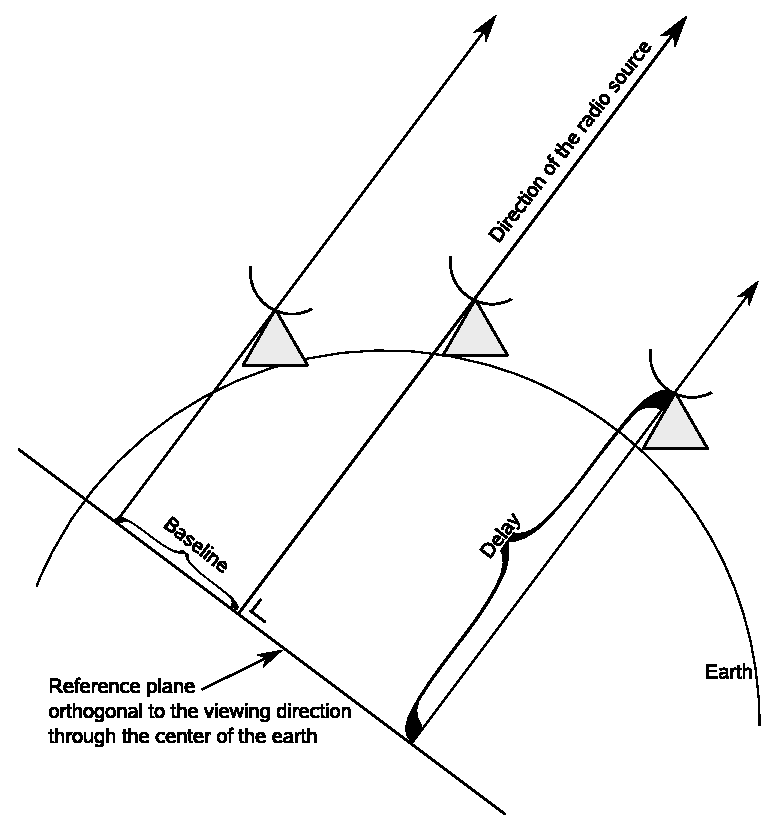
\includegraphics[width=.425\textwidth]
    {img/VLBI}
    \caption{Block diagram of the correlation.}
  \label{fig:correlation_diagram}
\end{figure}
\subsection{Correlation}
Correlation is the process by which data from multiple telescopes is
collected and combined to measure the spatial Fourier components of
the image of the sky. The high data rates and the optimizations
complicate the process.

Assume that we are correlating the signal of two telescopes. First,
both signals are delayed to account for the different time at which
the signal arrives at the telescopes, see
Figure~\ref{fig:correlation_diagram}. Next, a phase shift is performed
to compensate for the Doppler effect produced by the rotation of the
earth. This process requires very accurate timing information in the
data and a very detailed model of the geometry of the experiment. The
signals are now ready to be correlated.

During correlation, the first signal is delayed with discrete steps
and each delayed signal is multiplied with the second signal and then
integrated.  The output is a summation per delay step.

For more than two stations, each station is correlated with itself
(auto-correlation) and every other station (cross-correlation). Note
that the complexity is quadratic in the number of telescopes.


\section{VLBI}\label{sec:vlbi}
To achieve larger and larger resolution in astronomical imaging, it is
necessary to build larger telescopes, or to revert to
interferometry. As interferometry combines the measurements of several
telescopes to simulate a dish of a size equivalent to the maximal
distance between the farthest telescopes on the plane orthogonal to
the viewing direction. Numerous arrays (groups of telescopes) use this
technique, e.g., the VLA (Very Large Array), Lofar (Low-frequency
array), the EVN (European VLBI Network) or the VLBA (Very Large
Baseline Array).  Interferometry with telescopes that are
geographically very far apart is refered to as Very Large Baseline
Interferometry (VLBI). With VLBI it is possible to build a virtual
radio-telescope with a dish of size of the Earth. As the angular
resolution of a VLBI experiment depends on the maximal projected
distance between two radio-telescopes, VLBI achieves unsurpassed
angular resolution with the drawback of a relatively low sensitivity
\cite{VLBIbook}. Another important property is
sensitivity, as it allows to detect fainter astronomical
objects. Increasing the sensitivity is possible by adding more
radio-telescopes or by increasing the sampling rate or
resolution. Increasing the sampling rate or resolution increases the
data rate per telescope.

In order to get the final picture the signal gathered from the
radio-telescopes have to be correlated at a central place, the Joint
Institute for VLBI in Europe (JIVE).  JIVE is
operating a dedicated hardware correlator~\cite{EVNCorrelator}.

The maximal capacity of this hardware correlator is 16 telescopes at a
data rate of 1Gbs each. The requirements on both the data streams and
the computing power are shown in Table~\ref{tab:speed}.

% \marginpar{NGHK: Check 16Mb/s in table}
\begin{table}
  \centering
  \begin{tabular}[c]{|l|l|l|l|l|l|}
    \hline
    Description & \# & \#  & data-rate & spect/prod & Tflops\\
    & telescopes & sub-bands & (Mb/s) &  & \\
    \hline
    \hline
    Fabric-demo &4 &2 &16 &32 &0.16\\
    1 Gb/s, full array  &16 &16 &1024 &16 &83.39\\
    future VLBI &32 &32 &4096 &256 &\verb|~|21457\\
    \hline
  \end{tabular}
  \caption{Network bandwidths and computing power needed for an {\it e}-VLBI
    experiment based on a XF architecture.}
  \label{tab:speed}
\end{table}

\begin{figure}
  \centering 
  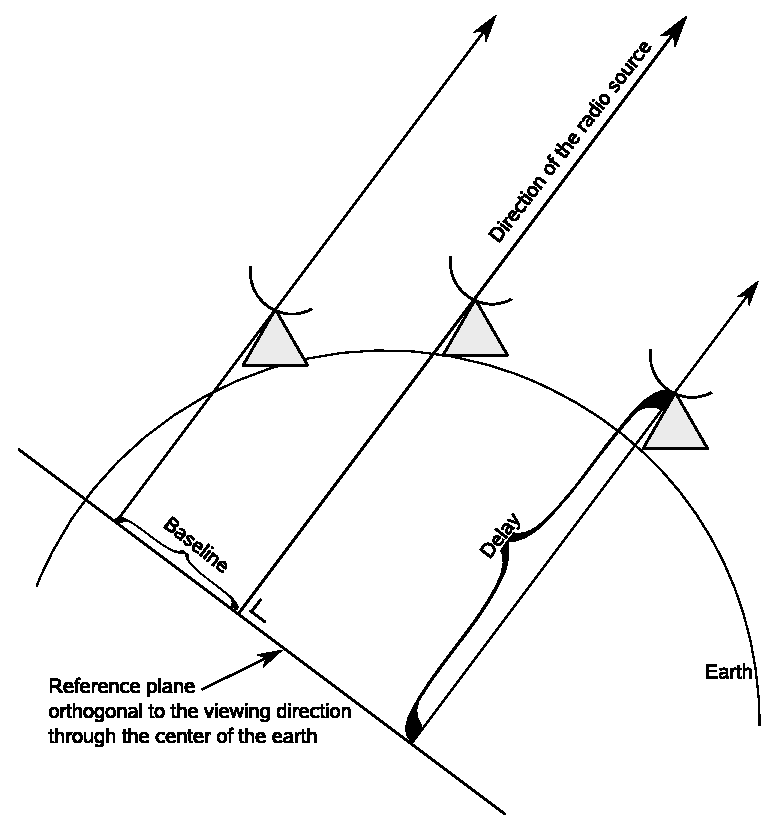
\includegraphics[width=0.5\textwidth]{img/VLBI.eps}
  \caption{Aligning the signals before correlation.}
  \label{fig:correlation_diagram}
\end{figure}

\paragraph{{\it e}-VLBI}
Traditionally, in VLBI, the data is recorded at the telescopes on disk
packs during an experiment. After the experiment the disks are shipped
to a central institute. There can be several weeks between the
experiment and the time when the correlated data becomes available.

Currently, JIVE is in the transition phase from traditional VLBI to
{\it e}-VLBI~\cite{szomoru-2004}. In an electronic VLBI ({\it e}-VLBI)
experiment, data from the telescopes is transferred directly over the
internet to JIVE, where it is streamed into the correlator in real
time. The data transport from the telescopes to JIVE goes over several
networks like local connections, paths provided by NRENs and the
G\'EANT backbone in Europe.

Transporting the data over the network has several advantages over a
traditional experiment. Obviously, the results of the experiments are
almost immediately available. This opens up the possibility to change
the course of an experiment based on earlier findings. Also, {\it
  e}-VLBI allows for real time analysis of the data and helps to
identify and resolve minor technical problems in the data collection
during the experiment.

Several experiments in the past have shown that real time {\it e}-VLBI
is possible. The EC funds the EXPReS project%
%\footnote{EXPReS is made
%  possible through the support of the European Commission (DG-INFSO),
%  Sixth Framework Programme, Contract \#026642.}
~\cite{EXPReS} which aims at building a production-level {\it e}-VLBI
instrument of upto 16 intercontinental telescopes connected in
real-time to JIVE and available to the general astronomy community.

\paragraph{Correlation}
Correlation is the process by which data from multiple telescopes is
collected and combined to measure the spatial Fourier components of
the image of the sky. It consists of two steps: first applying a delay
correction to align the signals and secondly computing the correlation
function for each pair of telescopes called a baseline.

To align the signals from the different telescopes, we project all the
telescopes on the plane through the center of the earth and orthogonal
to direction to the source, see
Figure~\ref{fig:correlation_diagram}. We will correlate the signals
received by the virtual projected telescopes. To compute these
signals, the signals from the real telescopes are delayed with the
distance between the telescope and its projection multiplied with the
speed of light (the signal travels with the speed of light). Note that
the delay changes during the observation because the earth rotates. We
conveniently split the delay in an integer number of samples and a
remaining fraction. While the integer delay is easily done by an
offset in the sample buffer, the fractional bit shift is usually
implemented as a phase rotation in the frequency domain. In a final
step, called the phase rotation, we change the sample rate to match
the rate of the delay function.

After the delay has been applied, the signals are ready for
correlation. Correlation~\cite{def_correlation} is mathematically
defined as a function on two signals in which the first signal is
delayed with discrete steps and the integral is computed of the
delayed signal multiplied with the second signal. The correlation is
done for each baseline (pair of telescopes). The correlation is called
an auto-correlation if the signal of a station is correlated with
itself and a cross-correlation if the signals are from different
stations. Note that the complexity of the correlation is quadratic in
the number of telescopes, as it is linear in the number of baselines.

To increase the signal to noise ratio, the correlated signal is
averaged over a certain period of time. Typical averaging times lie in
the range of $0.25-4$ seconds. Finally, the averaged signals are
Fourier transformed. Correlation in this order is refered to as XF,
because the correlation is done before the Fourier transform.  This is
how the correlation is implemented in most hardware correlators, as it
allows for large parallelisation.

One of the properties of correlation is that the Fourier transform of
two correlated signals is equal to multiplying the Fourier transformed
signals~\cite{corr_theorem}. This relation is used in most software
correlators, where correlation is more expensive than multiplication.
After the delay, the signal from each telescope is Fourier transformed
and the signals for each baseline are then multiplied elementwise.
This implementation is also refered to as FX: the Fourier transform comes
before the correlation.

%%% Local Variables:
%%% mode: latex
%%% TeX-master: "Ingrid"
%%% End:

\section{Software correlator}\label{sec:softwarecorrelation}
If the data in an {\it e}-VLBI experiment can be streamed over the
internet to JIVE, it can also be sent to another correlator. Within
\scarie, we are investigating the possibilities of a next generation
software correlator using a computing Grid. A similar attempt is
presented in \cite{deller-2007}. The advantages of a software
correlator over a new dedicated hardware correlator lies in its
flexibility and accuracy. The main advantage of a dedicated hardware
correlator is the greater performance. The flexibility of its
architecture allows the software correlator to change with the
individual needs of researchers. In fact, the first version of the
software correlator was developed to track the Huygens spacecraft
during its descent through the atmosphere of Saturn's moon Titan. Due
to the nature of this experiment, special requirements are put on the
correlator, which the current hardware correlator is not able to
provide.  Moreover, we expect that the costs of developing a software
correlator are much lower than the costs for a hardware correlator.

\begin{comment}
  The advance of general purpose computing is making software
  correlation a cost-effective solution for a range of applications.
\end{comment}

Currently, the software correlator is used in the production
environment for doing ftp-fringe tests for the EVN network. Since the
EVN is an ad-hoc array, the EVN telescopes are reconnected before
every VLBI-session. In order to test the EVN network, a ftp-fringe
test is done in which the telescopes observe a well known source and
transmit the data to JIVE where it is processed immediately. The
ftp-fringe tests provide quick feedback to the stations on their
performance.

Computationally the correlation is relatively inexpensive, in the
sense that it requires only few operations per received byte.
However, due to the high data rates, the absolute number of flops
(approximately 3Tflops) required by the application is still extremely
high for computing grids.  Moreover, the problem is quadratic in the
number of telescopes participating in the experiment since it is
linear in the number of channel pairs that have to be correlated. The
huge need for networking and computing power together with it's
flexibility, makes a cluster an good platform for this
application. Moreover, using grid technology the software correlator
can easily be executed on a large number of different clusters.



\begin{figure}
  \centering
  \includegraphics[width=.75\textwidth]
    {img/Network_correlator}
    \caption{Outline of the network connections between different
      components in the software correlator.}
  \label{fig:netw_corr}
\end{figure}


\subsection{Design}
In the software correlator, we split the computation in time slices.
These time slices are processed in parallel (see
Figure~\ref{fig:netw_corr}). The assignment of time slices to
computing nodes is done by a unique manager node. For every telescope
there is a unique input node that receives the raw stream and converts
it into time slices. These time slices are sent to correlator nodes
which do the actual correlation. The size of the output of the
correlation is much smaller than the input size and is collected and
stored by a single output node.

The manager node is the central node that controls the workflow of the
entire software correlator. It assigns time slices to available
correlator nodes and handles errors.

The input node receives the data from a data stream, which can either
be a file, a TCP connection or directly from the dedicated hardware
used to record and play back the data. It performs the integer delay
correction and then sends the data to the proper correlator node.

The correlator node gets data for the same time slice from every input
node. First it, compensates for the fractional delay and performs the
phase rotation. These manipulations are not done on the input node
because they require floating point samples, hence the data stream
expands from 2 bits per sample to 32 bits or even 64 bits per sample,
which would require much more network bandwidth. After the fractional
delay correction and the phase rotation, the signal is ready to be
correlated.  The auto and cross correlation are then computed by
Fourier transforming the input signal and element-wise multiplying all
baselines. These values are accumulated over a certain period of time
and the accumulated values are sent to the output node.

The output node will receives the data from the correlator nodes,
sorts the data and stores it at a specified location.

%%% Local Variables:
%%% mode: latex
%%% TeX-master: "Ingrid"
%%% End:

%\input{data_flow.tex}
\section{Execution and deployment.}\label{sec:network}
In section \ref{sec:vlbi} we presented the two operational 
mode we are targeting for the software correlator: \emph{batch-execution} 
and \emph{real-time}. Batch execution correspond to what the most common 
high performance computing scenario. If we except the \emph{size} 
of problem described in Section~\ref{sec:vlbi} and the 
challenge of making an efficient distributed application 
Section~\ref{sec:softwarecorrelation}, we consider that it is now relatively 
easy to run \emph{batch} job on top of existing grids 
infrastructure and middleware. Running the same \scarie~in a 
\emph{real-time} mode is much more complex as the grid 
infrastructure and corresponding middleware have to provide 
guarantees on the Quality of the Service that match 
the application's requirement. As these issues are still 
evolving rapidely we are testing these aspects of \scarie on 
an experimental grid called DAS-3 and its associated network 
service called StarPlane.

\subsection{Real-time and quality of service}
The term \emph{real-time} has a lot of definition in the computer science community, 
in this paper we will consider that a \emph{real-time} computation is a computation 
in which: \emph{the amount of buffering for an infinitely long experiment 
will only require a finite amount of buffers}. This is a formal way to define 
a process in which the incoming data are "consumed" by the computation 
as fast as they are generated. This definition also imply that once 
the application is started the allocated "space" on the resources will 
be maintained during the complete execution. 

The major resources \scarie is using are: the networking bandwidth, 
the computation resource and the disk-space if the data have 
to be saved. The sharing of the computational resource is now
a well understood process. Most of the time it is part of the 
execution service, this service taking a description of the 
application deployment as well as a description of the 
requested service (and resource). The execution service 
allocating rights to access the requested services or 
resource and, finally, if all part of the request 
are fulfilled, deploy the application. 
\begin{figure}
  \centering
  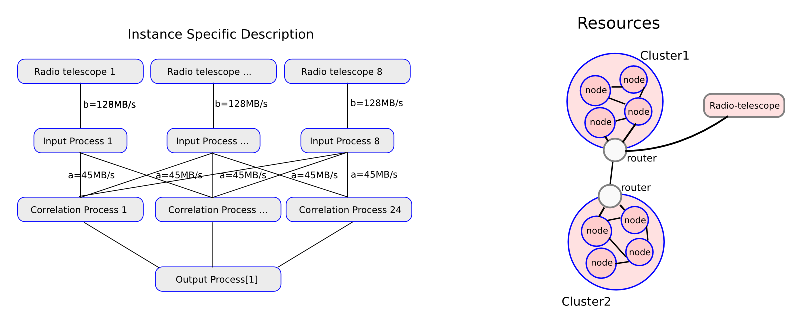
\includegraphics[width=\textwidth]
    {img/mapping.eps}
    \caption{Left: An specific instance of an experiment. Right: The resource set. Resource 
allocation and application scheduling have to map the left side to the resources. }
  \label{fig:mapping}
\end{figure}
The simplest way to offer guaranteed service over a shared resource consist
can be done restricting the access to only one user at a time. This approach is 
used in the DAS-3 grid (based on SGE) in which a node allocated is simply unusable 
by other users. Same principle could be applied to the complete grid including its 
networks and other resources. A more complicated, but really interesting approach 
consist of sharing the resource under the arbitration of a third party that will 
insure that each application is using only the allocated part of the resource. This 
is the approach that is often refereed in bibliography as Layer-2/3 QoS for 
network services, or the recently added Completely Fair Scheduler (per application 
control on their cpu usage) or IO- (per application IO-bandwith arbitration). In a 
very general point of view all these technology permit to virtualize the resource thus 
permit to build on top of a real grid a complete virtual environment based on user 
requirement.

\subsection{Running \scarie on \das3 and Starplane}
Networking issues are one of the challenges of the \scarie project. 
The regular Internet best-effort Layer3 IP routing has great
flexibility but is slow and unpredictable; on the other hand,
dedicated \textit{lightpaths} as available in 
\textit{lambda Grids}~\cite{eslea-2007}, with their predictable delays and
throughputs offer good performances and guarantee on the Quality of
Service (QoS). This is the approach that is used in \scarie to delivered 
the data from the radio-telescope to the 
computation center. Giving end user an access
to dedicated connection has been implemented in many of the current
research and education networks. The Dutch National Resarch and
Education network SURFnet is one of them. SURFnet6 deploys multiple
fiber optic rings that connect the academic and research locations
around The Netherlands. 

For the correlation process we are making experiment on the \das3 
grid. The \das3\ supercomputer~\cite{das3} was deployed in the summer of
2007. It is composed of fives clusters located in the Netherlands and
connected by an photonic network called StarPlane. StarPlane is also a
research project funded by the Netherlands Organization for Scientific
Research (NWO) and carried out at two Dutch Universities: the
University of Amsterdam (UvA) and the Vrije Universiteit Amsterdam
(VU). The goals of the project is to build an \textit{application-controlled 
photonic network}. StarPlane manage eight wavelengths in one of the SURFnet6 
optical rings. The originality of the StarPlane project 
is in its attempt to build a virtual network service at the lowest possible networking 
layer. This have the advantage to improve performances and to dramatically 
reduce the cost (the price or the energy) per byte transfered \cite{}. 
A complete virtual network for an application can then be build using only
vlan-on-mac layer 2 switches and layer-1 photonic lighpath. The other originality 
is that the photonic lightpath can dynamically be reorganized to adapt to the
user-application requests. 


\subsection{Benchmarks on DAS-3}
\scarie~ and StarPlane have parallel roadmap and thus the complete 
approach cannot be tested yet. We have conducted correlator performances test 
using \das3. The current software correlator is actually able to 
perform a 4x128Mbps experiment at 20\% of the real-time speed using a total of 16 (quad core 2.0Ghz cpu) nodes. 

In parrallel to correlation test we are working on the real-time based on 
the on demand virtual service. The only part of the StarPlane that is working at the time of writing is user-requestable lighpath service of StarPlane that permit to build and 
allocate a lighpath between two clusters. We tested this feature by running 
two client-server applications transmitting data between cluster. The communication middleware detect this scenario and allocate a lighpath, while the the lighpath is not availablethe application is sending the traffic to the normal network interface; when it become ready the traffic is switched to the lighpaths.  
\begin{figure}[h]
  \centering
  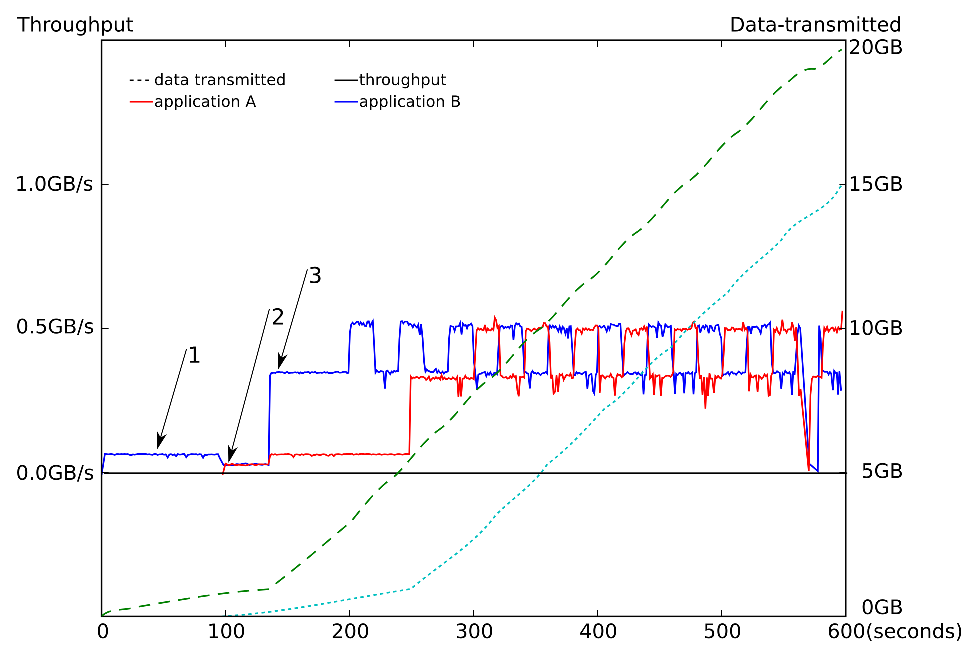
\includegraphics[width=\textwidth] {img/timing.eps}
    \caption{\label{fig:timing}
		Two application executed on the StarPlane network. The application share the ethernet part of the network. Then acquire a lighpath, the change of the bandwith is clearly sensible.}
\end{figure} 

This experiment rise questions, as the supposly secured path that is suppose to deliver reliably "550MB/s" of throughput between a pair of cluster. In Figure~\ref{fig:timing} we can see a periodic artifact, the traffic falling down to 300MB/s for few seconds. A second to investigate issue is that from time to time the lighpath connectivity disapear and these issue have to be investigated in order to provide a "real" guaranteed service. 

%\section{Benchmarks}\label{sec:benchmarks}

%%% Local Variables:
%%% mode: latex
%%% TeX-master: "Ingrid"
%%% End:

\section{Conclusion and future work}\label{sec:conclusion}
In the last year we laid the foundation for a flexible software
correlator based on distributed computing technologies. \acomment{Damien: }{Saying that it is now deliverable state.} Using this
software correlator we are currently collaborating intensively with
the StarPlane project in order to test incoming network with
guarenteed Quality of Services for grid.

\paragraph{Future work}
Within \scarie\ and a related project FABRIC, which is a joint
research activity in the EXPR{\it e}S project, we are currently
improving and testing more intensively the software correlator. \acomment{Damien:}{ 
Saying we can see several way to improve the speed at at least 6x. }

On the batch processing aspect of \scarie~ we want to investigate 
how dynamical resources can be added during the application run time to 
accelerate the computation. This include node joining/leaving the calculus as well as
setting up lighpath between input-nodes and the joining nodes.

We also want to continue our testing on the traffic isolation features of
the incoming networks as the one provided by Starplane. This include
interaction with network service providers as well as on experiencing
networking protocols to optimize the data transfer (using UDP instead
of TCP).

\section{Acknowledgment}
\scarie\ is a joint research project of JIVE, the UvA and SARA funded
by the Netherlands Organization for Scientific Research (NWO).



%%% Local Variables:
%%% mode: latex
%%% TeX-master: "Ingrid"
%%% End:


% BibTeX users please use
\bibliographystyle{plain}
\bibliography{biblio}

%\ifodd\thepage
%\newpage
%\thispagestyle{empty}
%\centerline{\hfill}
%\fi
\end{document}

